This section introduces the relevant theory required for this experiment. The amount of rigor is only what is required for understanding the concepts. Further information can be found in \cite{mes}, unless a different source is cited.

\section{Generation of Harmonics}
Any arbitrary potential $V$ can be approximated by a harmonic potential at its minima. Depending on the order of approximation, this would suit majority of the problems. But such a treatment would break down when the approximation is no longer accurate to describe the system. In such cases, we need to include higher order potentials. This is, ultimately, the essence of perturbation theory. Suppose, we have a system of atoms irradiated with some source of light. Depending on the intensity of the source, the effects might completely be linear (which corresponds to a harmonic potential). For example, a linear effect would be the one in which the polarisation vector, $P$ is directly proportional to the electric field, $E$. But when you have an anharmonic potential, the linear proportionality no longer holds. In such cases, we need to include higher order effects. This can be done by expanding in terms of the field,
\begin{equation}
    \bm{P} = \epsilon_0 \left( \chi^{(1)} \bm{E} + \chi^{(2)} \bm{E_1E_2} + \mathcal{O}\bm{(E^3)} \right),
\end{equation}
where we have considered up to second order effects. The $\chi(n)$'s are a rank $(n+1)$ tensor, which relate the effect of Electric field on the polarization vector. For the first term, it reduces to the linear susceptibility of the medium. For an electric field corresponding to an incoming plane wave, which is the case of an incoming photon, the second order effect on the polarization is given by,
\begin{equation}
    P^{(2)} = \epsilon_0 \chi^{(2)} E_0^2 sin^2(\omega t) = \frac{1}{2} \epsilon_0 \chi^{(2)} E_0^2 (1 - cos(2\omega t)),
\end{equation}
where the plane wave is taken to be of the form $\lvert \bm{E} \rvert = E_0 sin(\omega t)$. We can see from the above equation that the addition of second order effect leads to the generation of a wave of double the frequency plus a constant term, which can be seen as a constant shift in the overall polarization of the medium. We call the first order effect, which is a beam corresponding to the same frequency as the fundamental beam and the second order effect, which is a beam corresponding to double the frequency as the second harmonic. The intensity of the second harmonic then is related to the fundamental beam by,
\begin{equation}
    I_{SH} = I_{FUN}^2 \Gamma^2 L^2 sinc^2(\Delta k L),
\end{equation}
where $\Gamma$ depends on the medium, $L$ is the length of the medium traversed by the beam and $\Delta k = \frac{2\omega}{c}(n(2\omega)-n(\omega))$, is known as the phase mismatch. Also here, $sinc(x) = \frac{sin(x)}{x}$, attains its maximum value when the argument is zero. Therefore, we have to carry out a so called ``phase-matching'' to maximise the intensity of the second harmonic beam. This mismatch, as it can been seen from the equation, arises due to the dependence of the refractive index on the frequency.

\section{Birefringence and Retarder Plates}
We noted in the previous section that the refractive index depends on the frequency. Generally, it also depends on the direction of propagation of the wave. Isotropic media are special materials which don't have any directional dependence of refractive index. Hence the name, ``isotropic''. The most general materials, whose refractive indices depend on the direction of propagation of wave, are called birefringent. Uniaxial crystals are a particular type of birefringent material that have two unique refractive indices. They have one \textit{extraordinary} and two \textit{ordinary} directions. For a beam polarised along the extraordinary direction, also called the optical axis of the crystal, the beam will experience a refractive index of $n_e$. Whereas, for polarisation along the ordinary directions, the beam will experience a refractive index of $n_o$. For any other direction, the effective refractive index will be a combination of these two refractive indices. For a beam passing through the crystal with an angle $\theta$ with the ordinary axis, the effective refractive index is given by,
\begin{equation}
    \frac{1}{n_{eff}^2(\theta)} = \frac{cos^2\theta}{n_o^2} + \frac{sin^2\theta}{n_e^2}.
\end{equation}
This is an equation of an ellipsoid. The case where ($n_o < n_e$) is called negative birefringence and the case where ($n_o > n_e$) is called positive birefringence.\\
The above property is quite exotic and lets us explore different applications. One such application is the waveplates or the retarder plates, which are constructed using birefringent materials. These are used to change the polarisation of an incident wave. There are two kinds of waveplates. A $\lambda/2$ plate rotates the polarisation direction by an angle $2\phi$ for an incident wave with an angle $\phi$ between the optical axis and the polarisation. A $\lambda/4$ plate is used to produce circularly polarised light from a linearly polarised light by having the angle between polarisation and optical axis as $45^{\circ}$. For other angles, it produces and eliptically polarised light. It can also be used to produce a linearly polarised light from a circularly polarised light.

\section{Phase Matching}
As mentioned in the previous sections, to maximise the intensity of the second harmonic, we would like to carry out \textit{phase matching}. As noted earlier, this factor arises due to the fact that the phase of the different waves involved will not necessarily change in the same way as they pass through a material. This irregularity will then result in an interference that either constructs or destructs the final result. Ultimately, we would like to make the factor $\Delta k$, noted in section \textit{Generation of Harmonic}, as close to zero as possible. To do this, we discuss methods that use birefringence here.

\subsection{Type I Phase Matching}
This is the most straightforward method to understand. We change the orientation of the crystal in such a way that, for a material with positive birefringence, the second harmonic passes through the ordinary axis and the fundamental wave passes through an axis perpendicular to it. In the case of material with negative birefringence, the second harmonic is made to pass through the extraordinary axis and the fundamental wave through an axis perpendicular to it. Now, if the constants of the material are chosen properly, we can achieve phase matching, $n_o (2\omega) = n_e (\omega)$. Even though this method can be understood easily, it is not very easy to perform since we have to carefully tune the material constants.

\subsection{Type II Phase Matching}
To overcome the problem of carefully tuning the material constants, we could opt for type II phase matching. This depends on the fact that the effective refractive index of an uniaxial material is an equation for an ellipsoid. By taking the ellipsoids for both the fundamental wave and the second harmonic and by finding the point at which they intersect, we can achieve phase matching. The points at which they intersect correspond to exact phase matching, $n_o(2\omega, \theta) = n_e(\omega, \theta)$, for a positive birefringent material and the opposite for a negative birefringent material. This method is illustrate in the figure \ref{fig:phasematching}.\\
\begin{figure}[h!]
\centering
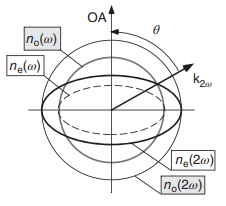
\includegraphics[width = 6 cm]{phase-matching.png}
\caption{Illustration of type II phase matching - points of intersection for different ellipsoids\ref{mes}}
\label{fig:phasematching}
\end{figure}
Even though this method is neater than the previous method, it still has one drawback just like the previous method. It is sensitive to the value of the theta, i.e., the orientation. Hence, these methods together are also called critical phase matching.

\subsection{Non-critical Phase Matching}
In a non-critical phase matching, we try to achieve phase matching through methods that don't depend on the angle. One such way is to change the temperature of the material to achieve phase matching. This is not used separately, but rather used in tandem with the critical methods. The critical methods are used to achieve a rough phase matching and then the temperature of the crystal is varied to achieve finer phase matching.

